
\section{Dam break on wet areas}

The dam break problem on wet areas was solved analytically by Stoker~\cite{Stoker1948, Stoker1957}. The analytical solution exhibits a rarefaction and involves a shock. Generally this problem is easier to solve numerically than the dry dam break (the dam break on a dry area).

The initial condition is
\begin{equation} \label{eq:dbp_init_wet}
u(x,0)=0, ~~v(x,y)=0, ~~\textrm{and}~~
h(x,0) = \left\{ \begin{array}{ll}
h_1 & \textrm{if $x < 0$}\\
h_0 & \textrm{if $x > 0$}\\
\end{array} \right.
\end{equation}
where $h_1>h_0>0$. The topography is a horizontal flat bed.

The analytical solution~\cite{Stoker1948, Stoker1957} to the wet dam break problem is
\begin{equation}
h(x) = \left\{ \begin{array}{ll}
h_1 & \textrm{if $x \leq -t \sqrt{gh_1}$}\\
h_3=\frac{4}{9g}(\sqrt{gh_1}-\frac{x}{2t})^2 & \textrm{if $-t \sqrt{gh_1} <x \leq t(u_2-\sqrt{gh_2}$})\\
h_2=\frac{h_0}{2}\bigg(\sqrt{1+\frac{8\dot{\xi}^2}{gh_0}}-1\bigg) & \textrm{if $ t(u_2-\sqrt{gh_2}) <x < t\dot{\xi}$}\\
h_0 & \textrm{if $x \geq t\dot{\xi}$}\\
\end{array} \right.
\end{equation}
and
\begin{equation}
u(x) = \left\{ \begin{array}{ll}
0 & \textrm{if $x \leq -t \sqrt{gh_1}$}\\
u_3=\frac{2}{3}(\sqrt{gh_1}+\frac{x}{t}) & \textrm{if $-t \sqrt{gh_1} <x \leq t(u_2-\sqrt{gh_2}$})\\
u_2=\dot{\xi}-\frac{gh_0}{4\dot{\xi}}\bigg(1+\sqrt{1+\frac{8\dot{\xi}^2}{gh_0}} \bigg) & \textrm{if $ t(u_2-\sqrt{gh_2}) <x < t\dot{\xi}$}\\
0 & \textrm{if $x \geq t\dot{\xi}$}\\
\end{array} \right.
\end{equation}
at any time $t>0$, where $\dot{\xi}$ is the shock speed constant given by 
\begin{equation} \label{eq:shock}
\dot{\xi}=2\sqrt{gh_1}+\frac{gh_0}{4\dot{\xi}}\bigg( 1+\sqrt{1+\frac{8\dot{\xi}^2}{gh_0}}\bigg)-\bigg( 2gh_0 \sqrt{1+\frac{8\dot{\xi}^2}{gh_0}}-2gh_0\bigg)^\frac{1}{2}.
\end{equation}


\subsection{Results}

For our test, we consider $h_1=10$ and $h_0=1$ in (\ref{eq:dbp_init_wet}).
The following figures show the stage, $x$-momentum, and $x$-velocity at several instants of time.
We should see excellent agreement between the analytical and numerical solutions. 

\begin{figure}[h]
\begin{center}
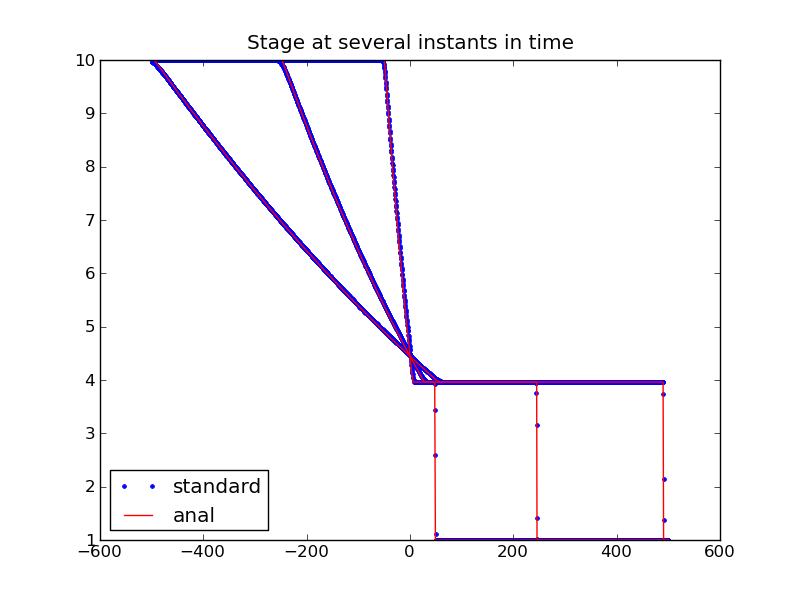
\includegraphics[width=0.9\textwidth]{stage_plot.png}
\end{center}
\caption{Stage results}
\end{figure}


\begin{figure}[h]
\begin{center}
\includegraphics[width=0.9\textwidth]{xmom_plot.png}
\end{center}
\caption{Xmomentum results}
\end{figure}


\begin{figure}[h]
\begin{center}
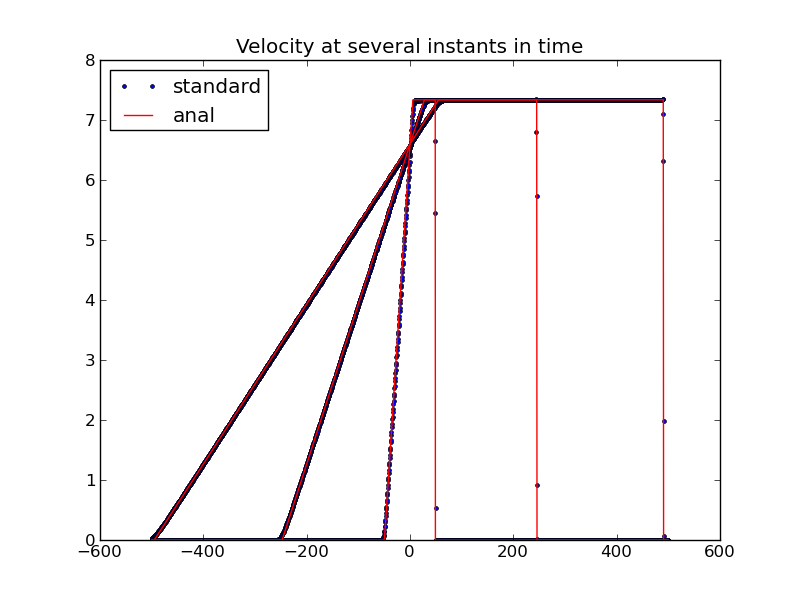
\includegraphics[width=0.9\textwidth]{xvel_plot.png}
\end{center}
\caption{Xvelocity results}
\end{figure}


\endinput
